\renewcommand{\lastmod}{20. Dezember 2024}
\renewcommand{\chapterauthors}{Markus Lippitz}

\chapter{Rotation und Schwingung in Molekülen}



\section{Überblick}


In diesem Kapitel behandeln wir die Spektroskopie von Molekülen mit dem Ziel, die Eigenschaften des Bindungspotentials zu bestimmen. Wir beginnen mit einem allgemeinen, spektral sehr breiten Überblick über die spektroskopischen Eigenschaften von Molekülen, die in ihren dielektrischen Eigenschaften zum Ausdruck kommen. Die dielektrische 'Konstante' kann als eine Summe von Lorentz-Oszillatoren dargestellt werden.  Jeder Oszillator, jede Resonanz entspricht einem Freiheitsgrad des Moleküls. In diesem Kapitel werden Rotationen und Schwingungen behandelt, im nächsten Kapitel die elektronische Anregung. Elektronische Anregung ist die Anregung, die wir schon bei den Atomen besprochen haben. Aber nur Moleküle, die aus mehr als einem Atom bestehen, können gegeneinander schwingen oder sich drehen.

Der zweite Abschnitt dieses Kapitels befasst sich daher mit den Rotationen der Moleküle und wie sie sich im Spektrum widerspiegeln. Wir werden sehen, dass Rotationen im Modell des starren Rotators zu einer Reihe von äquidistanten Linien mit einer charakteristischen Amplitudenverteilung führen.

Ein schwingendes Molekül zeigt zunächst nur eine Linie im Spektrum. In Kombination mit der Rotation entstehen jedoch weitere Linien, wenn sich bei einem optischen Übergang die Rotationsquantenzahl und die Schwingungsquantenzahl gleichzeitig ändern. Schließlich versuchen wir, die Vielzahl möglicher Schwingungen in mehratomigen Molekülen zu beschreiben.


\section{I Beispiel: Wasser}

\begin{figure}
\inputtikz{\currfiledir fig_water}
\caption{Dielektrische Funktion $\epsilon = \epsilon' - i \, \epsilon''$ von flüssigem Wasser (\cite{Segelstein_water} via 
\href{https://refractiveindex.info/?shelf=main&book=H2O&page=Segelstein}{refractiveindex.info}). Der niederfrequente Bereich unterhalb von $\bar{\nu} = 30$~cm$^{-1}$ ist um den Faktor 20 reduziert dargestellt.
\label{fig:diel_water}}

%D. J. Segelstein. The complex refractive index of water, Master Thesis (1981)
%https://refractiveindex.info/?shelf=main&book=H2O&page=Segelstein
% http://hdl.handle.net/10355/11599 
\end{figure}


Das in Abbildung \ref{fig:diel_water}  gezeigte Spektrum von flüssigem Wasser überdeckt mehr als 6 Größenordnungen im Frequenzbereich und ist mit einem einzigen Gerät nicht  messbar. Die niedrigsten Frequenzen liegen im Bereich von Mikrowellen, benutzt also Techniken aus dem Radio- und Radar-Bereich. Der mittlere Frequenzbereich ist infrarotes Licht, der hohe sichtbares bis ultraviolettes Licht. Wir werden die verschiedenen spektroskopischen Methoden in diesem und dem nächsten  Kapitel besprechen.


Die Wellenzahl $\bar{\nu} = 1 / \lambda =\nu / c =  E / (h c)$ (eigentlich immer angegeben in der Einheit 1/cm) ist eine Maß für die  \emph{Frequenz} oder \emph{Energie}. Dieses Maß in der Spektroskopie sehr weit verbreitet ist, weil es proportional zur Energie ist (und damit das Reziproke der Wellenlänge umgeht), aber gleichzeitig nahe an der praktischen, intuitiven Größe 'Wellenlänge'.



% \begin{questions} 
% \item Wo in  Abbildung  \ref{fig:diel_water} ist der sichtbare Spektralbereich, wo die Frequenz von Radio Mainwelle?
% \end{questions}

Wie kommt es aber nun zu diesem Spektrum? Wenn wir ein Stück dielektrische Materie in einen Plattenkondensator halten, dann bewegt das elektrische Feld $\mathbf{E}$ des Kondensators die Ladungsträger der Ladung $q$ in der Materie um  die Distanz $\Delta  \mathbf{x}$ von der neutralisierenden Gegenladung $-q$ weg. Dadurch entsteht dadurch ein Dipolmoment $\mathbf{p} = q \Delta \mathbf{x}$. Oft werden Dipolmomente in der Einheit Debye angegeben ($1 D = 3{,}33564 \cdot 10^{-30}$ C  m). Ein Elektron im Abstand von 1~\AA\ von einem Proton produziert ein Dipolmoment von etwa 4.8~D. Bei $N$ Molekülen (Ladungsträgerpaaren) pro Volumen ergibt sich eine makroskopische Polarisation $\mathbf{P}$ zu
\begin{equation}
\mathbf{P} = N \, q \, \Delta \mathbf{x} = f(\mathbf{E}) \quad .
\end{equation}
Der Zusammenhang zwischen angelegtem externen Feld $\mathbf{E}$ und resultierende 
Polarisation $\mathbf{P}$ hängt ganz entscheidend vom mikroskopischen Aufbau der Materie ab. Alle Methoden der Spektroskopie vermessen diesen Zusammenhang. Oft wird er als 
\begin{equation}
 \mathbf{P} =  (\epsilon - 1) \, \epsilon_0 \, \mathbf{E} = \epsilon_0 \,\chi \, \mathbf{E} 
 \label{eq:diel_p_lin}
\end{equation}
geschrieben, mit der relativen Permittivität\sidenote{Vorsicht, hier gibt es verschiedene Schreibweisen. Ich benutze die Form $D = \epsilon \epsilon_0 E$, mit einheiten-freiem $\epsilon$. Manchmal findet man $\epsilon_0 \epsilon_r$, manchmal auch nur $\epsilon$.} $\epsilon$ bzw. der elektrischen Suszeptibilität $\chi$. 


Die Aussage von Abbildung \ref{fig:diel_water} ist, dass die  dielektrische 'Konstante' $\epsilon$   nicht  konstant ist, sondern eine dielektrische Funktion der Frequenz, also $\epsilon(\nu)$. Verschiedene Prozesse tragen zur Frequenzabhängigkeit bei:




\paragraph{Orientierungspolarisation} Die Orientierung des Moleküls im Feld ist eine Drehbewegung. Diese Bewegungen werden bei der \emph{Rotationsspektroskopie} unten detaillierter behandelt werden. Hier greifen wir vor. Der Drehimpuls $L$ ist in der Quantenmechanik quantisiert. Sei
\begin{equation}
1 \hbar = L = J \, \omega = m_\text{red} \, R^2 \, \omega
\end{equation}
mit dem Trägheitsmoment $J$, der Kreisfrequenz $\omega$ und der reduzierten Masse 
 $m_\text{red}$ sowie dem Bindungsabstand $R$ in einem angenommenen zwei-atomigen Molekül. Für das Molekül HCl gilt $R = 1.28$~\AA\ und $m_\text{red} \approx m_H = 1$~u. Damit ergibt sich eine Frequenz $\nu = 628$ GHz, also im Mikrowellen-Bereich. Oft wird dies auch geschrieben als Wellenzahl $\bar{\nu} = 1 /\lambda \approx 10$~cm$^{-1}$.
 
\paragraph{Verschiebung der Kerne} Bei der Verschiebungspolarisation können sich zunächst einmal die Kerne bzw. Ionen gegeneinander bewegen. Dies ist Thema der \emph{Schwingungsspektroskopie}, und wieder greifen wir vor. Zwei Atome seien im Gleichgewicht  im Bindungs-Abstand $R_0$. Wir nehmen an, die Rückstellkraft in diesem Gleichgewicht sein allein die Coulomb-Kraft des einen Kerns auf den anderen, also 
\begin{equation}
F = \frac{1}{4 \pi \epsilon_0} \, \frac{e^2}{R^2} \quad .
\end{equation}
Die Federkonstante $k$ ist dann die Ableitung dieser Kraft nach $R$. Für das Molekül HCl mit einem Gleichgewichts-Abstand $R_0 = 1.2$~\AA\ ergibt sich $k = 220$~N/m. Die Eigenfrequenz der Schwingung  ist $\nu = (1/2\pi) \, \sqrt{k/m_\text{red}} = 58$~THz mit der reduzierten Masse von oben. Dies entspricht einer Wellenlänge von $\lambda = 5.12$~\textmu m, also im Infraroten, und einer Wellenzahl $\bar{\nu} = 2000$~cm$^{-1}$.

\paragraph{Verschiebung der Elektronenwolke} Wenn es zu einer Resonanz in der Verschiebung der Elektronenwolke kommt, dann entspricht dies einer \emph{elektronischen Anregung}, also einem quantenmechanischen Übergang zwischen zwei Elektronen-Orbitalen. Dies wird uns  im nächsten Kapitel beschäftigen. Wir schätzen hier die Übergangsenergie analog zu atomaren Übergängen ab
\begin{equation}
  h \nu = hc \, R_H \, \left( \frac{1}{n^2} - \frac{1}{m^2} \right) \quad .
\end{equation}
Für Atome liegt die Frequenz $\nu$ im Bereich von $10^{15}$~Hz $= 1$~PHz. Bei Molekülen liegt sie etwas niedriger, also $\nu \approx 10^{14} \cdots 10^{15}$~Hz, also $100 \cdots 1000$~THz.


\section{Lorentz-Oszillator-Modell}


\begin{marginfigure}
\inputtikz{\currfiledir lorentz_oszillator}

\caption{Frequenzabhängigkeit des Real- und Imaginärteils des Lorentz-Oszillators. Real- und  Imaginärteil des komplexwertigen Brechungsindex $\tilde{n}$ sehen qualitativ gleich aus. \label{fig:diel_lorentz}}
\end{marginfigure}

Alle oben diskutieren Phänomene sind Resonanzen. Das Lorentz-Oszillator-Modell ist ein einfaches Modell, mit dem die Frequenzabhängigkeit der dielektrischen Funktion in der Nähe solcher Resonanzen beschrieben werden kann. In einem gedämpften harmonischen Oszillator (Masse $m$, Dämpfungskonstante $\gamma$, Eigenfrequenz $\omega_0$) wird die Masse durch ein periodisches elektrisches Feld (Amplitude $E_0$, Frequenz $\omega$) um $x$ ausgelenkt, da die Masse eine Ladung $e$ trägt. Alles zusammen
\begin{equation}
 m \ddot{x} +  \gamma \dot{x} + m \omega_0^2  x = e E_0 e^{+ i \omega t} \quad .
\end{equation}
Die stationäre Lösung dieser Differentialgleichung ist
\begin{equation}
 x(t) =  \frac{e \, E_0}{m (\omega_0^2  - \omega^2) + i \gamma \omega} \, e^{+ i \omega t} \quad .
\end{equation}
Die makroskopische Polarisation $P$ ist die Summe über alle mikroskopische Polarisationen, also
\begin{equation}
P(t) = N \, e \,x(t) =  (\epsilon -1 ) \epsilon_0 \, E_0 e^{+ i \omega t}
= \chi \epsilon_0 E(t) \quad .
\end{equation}
Damit ergibt sich die dielektrische Funktion
\begin{equation}
\epsilon(\omega) = 1 + N \alpha = 1 +\frac{N e^2}{\epsilon_0} \frac{1}{m (\omega_0^2  - \omega^2) + i \gamma \omega} = \epsilon' - i \epsilon'' \quad .
\end{equation}
Man beachten das per Konvention negative Vorzeichen des Imaginärteils $\epsilon''$. Explizit sind Real- und Imaginärteil
\begin{align}
 \epsilon' = & 1 + \frac{N e^2}{\epsilon_0} \frac{ m (\omega_0^2  - \omega^2)}{m^2 (\omega_0^2  - \omega^2)^2 +  \gamma^2 \omega^2}  \\
  \epsilon'' = &  \frac{N e^2}{\epsilon_0} \frac{ \gamma \omega }{m^2 (\omega_0^2  - \omega^2)^2 +  \gamma^2 \omega^2}  \quad .
\end{align}
Für den  komplexwertige\sidenote{Oft wird nicht zwischen $n$ und $\tilde{n}$ unterschieden und $n$ selbst ist komplexwertig.} Brechungsindex\sidenote{Die hier benutzte Konvention der Vorzeichen ist die in der Physik übliche, ausgehend von der Zeitabhängigkeit $e^{+ i \omega t}$. In der eher ingenieurwissenschaftlichen Literatur findet sich aber genauso oft auch die Zeitabhängigkeit $e^{- i \omega t}$. Dies führt zu komplex-konjugierten Gleichungen. } $\tilde{n} = n - i k$ gilt
\begin{align}
 \epsilon = & \tilde{n}^2 = (n - i k)^2 \\
  \epsilon' =& n^2 - k^2 \\
 \epsilon'' = & 2 n k \quad .
\end{align}
Dabei beschreibt $k$ die Dämpfung und $n$ die Dispersion, also die Variation der effektiven Wellenlänge in der Nähe einer Resonanz:
\begin{equation}
E(t,z) = E_0 \, e^{i \omega (t - \frac{z}{c}(n - i k))} = 
 E_0 \, e^{ - \frac{\omega}{c} k z}  
 \, e^{i \omega (t - \frac{z}{c/n} )}  \quad .
\end{equation}

Wenn in einem Medium mehrere Resonanzen vorhanden sind, so addieren sich die Suszeptibilitäten:
\begin{equation}
\epsilon(\omega)_\text{ges} = 1 + \chi(\omega)_\text{elec} +  \chi(\omega)_\text{ion}  + \chi(\omega)_\text{orient} \quad .
\end{equation}

\begin{marginfigure}
\inputtikz{\currfiledir multiple_lorentz_oszillator}

\caption{Addition der Suszeptibilitäten. \label{fig:diel_multiple_lorentz}}
\end{marginfigure}

Für Fensterglas liegt die elektronische Resonanz im Ultravioletten. Sichtbares Licht ist also im Frequenzbereich etwas unterhalb dieser Resonanz. Die sogenannte 'normale' Dispersion des Brechungsindex (ansteigend mit fallender Wellenlänge / steigender Frequenz) rührt gerade von dem Anstieg der dielektrischen Funktion zur elektronischen Resonanz hin her.



%%%%%%%%%%%%%%%%%%%%%%%%%%%%%%%%%%%%%%%%%%%%%%%%%


\section{II Rotation von Molekülen}




\begin{figure}
\inputtikz{\currfiledir fig_hcl}
\caption{Mikrowellen-Transmissionspektrum durch  \ch{HCl}-Gas  (\cite{Li_2011_hcl} via \href{https://hitran.org}{hitran.org}).
\label{fig:rot_hcl}}
\end{figure}




Der dargestellte Bereich  von etwa 10 bis 300 cm$^{-1}$ entspricht einer Frequenz von 0.3 bis 9 THz oder einer Wellenlänge von 1000 bis 33 \textmu m. Dieser Spektralbereich ist experimentell nicht einfach zugänglich (\emph{THz gap}). Für niedrigere Frequenzen unterhalb etwa 0.3 THz, im Mikrowellen-Bereich, existieren in der Frequenz durchstimmbare  Mikrowellen-Generatoren (Klystron) und passende Detektoren. Bei höheren Frequenzen ist dies technisch aufwändig. Möglichkeiten sind das Synchrotron oder durch sehr kurze Laserpulse erzeugte THz-Pulse.

Nach Erzeugung der Strahlung durch Klystron oder Synchrotron wird diese durch ein möglichst langes Volumen des zu untersuchenden Gases geleitet, da die Absorption gering ist. Die transmittierte Leistung wird dann als Funktion der Frequenz des Generators gemessen. So erhält man  Spektren ähnlich zu oben stehender Abbildung.

Die Transmission $T$ (oder auch die Absorption) ist eine etwas unpraktische Größe, da sie immer im Bereich zwischen Null und Eins liegt, also beispielsweise nicht linear von der Konzentration des Gases abhängt. Daher betrachtet man eigentlich immer die Absorbanz oder Extinktion.\sidenote{Der Unterschied zwischen Absorbanz und Extinktion ist, dass letztere auch Streuung beinhaltet, was für uns aber keine Rolle spielt.} Die Extinktion $E$ ist
%
\begin{equation}
 E = - \log_{10} T \quad .
\end{equation}
%
Im Folgenden betrachten wir also Absorbanz- oder Extinktions-Spektren, die oft auch einfach Absorptionsspektren genannt werden, auch wenn nicht $1-T$ sondern $\log_{10} ( 1- T)$ dargestellt ist.

\begin{marginfigure}
\inputtikz{\currfiledir fig_hcl_extinction}
\caption{Das HCl-Spektrum aus Abbildung \ref{fig:rot_hcl} als Extinktionsspektrum.}
\end{marginfigure}


% \begin{questions} 
% \item Wo in  Abbildung  \ref{fig:rot_hcl} arbeitet ein Mikrowellenherd?
% \end{questions}


\section{Modell des starren Rotators}

Ein einfaches Modell, um Rotationsspektren zu beschreiben, ist das des starren Rotators. Wir nehmen eine klassische Hantel mit zwei Massen $m_1$ und $m_2$ an, die durch eine starre Achse der Länge $R$ miteinander verbunden sind. Das Trägheitsmoment der Hantel ist
\begin{equation}
 \Theta = \frac{m_1 \, m_2}{m_1 + m_2} \, R^2 = m_\text{red} \, R^2 \quad .
\end{equation}
Damit berechnet sich die Rotationsenergie $E_\text{rot}$ zu
\begin{equation}
 E_\text{rot} = \frac{1}{2} \, \Theta \, \omega^2
\end{equation}
mit der Rotationsfrequenz $\omega$. Die Quantenmechanik kommt durch die Quantisierung des Drehimpulses $\mathbf{L} $ ins Spiel:
\begin{equation}
 | \mathbf{L} | = \Theta \, \omega = \hbar \sqrt{J (J + 1)}
\end{equation}
mit der Drehimpuls-Quantenzahl $J = 0, 1, \dots$. Die Rotationsenergie ist damit
\begin{equation}
 E_\text{rot} = \frac{ | \mathbf{L} |^2}{2 \Theta} = \frac{\hbar^2 \, J (J+1)}{2 \Theta} \quad .
\end{equation}

Dies sind die Energien der \emph{Zustände} des Systems, noch nicht die Lage der Peaks im Spektrum. Bei der Absorption eines Mikrowellen- oder THz-Photons ändert sich der Zustand. Wir suchen also die Energien der \emph{Übergänge} zwischen Zuständen, um die Lage der Peaks im Absorptionsspektrum zu beschreien.


% \begin{questions} 
% \item Um welche Achse dreht man die Hantel in diesem Modell?
% \end{questions}


\section{Auswahlregeln bei Rotationsübergängen}

Zwischen welchen Zuständen können unter welchen Umständen Übergänge durch Absorption (oder Emission) eines Photons stattfinden? Dies beschreiben  die Auswahlregeln.

Zunächst muss die Rotationsbewegung überhaupt an das elektromagnetische Feld koppeln. Dies verlangt  ein statisches, permanentes Dipolmoment des Moleküls. Klassisch hätte man so einen oszillierenden Dipol, und diese Bedingung bleibt auch in der Quantenmechanik erhalten. Damit sind homonukleare Moleküle (z.B. \ch{H2}), symmetrische lineare Moleküle (z.B. \ch{CO2}) und hoch-symmetrische Moleküle (z.B. \ch{CCl4}) ausgeschlossen. Dieser Ausschluss kann, wie wir unten sehen werden, durch eine Schwingung des Moleküls wieder aufgehoben werden.

Wenn optische Rotationsübergänge im Prinzip möglich sind, dann muss noch die Drehimpuls-Erhaltung erfüllt sein. Die Summe des Drehimpulses von Molekül und Photon muss erhalten bleiben. Der Drehimpuls des Photons ist $1 \hbar$. Bei der Absorption eines Photons muss sich also $J$ erhöhen, bei der Emission erniedrigen.\sidenote{Glücklicherweise passt das mit der Änderung der Energie zusammen.} Damit ergibt sich als Auswahlregel
\begin{equation}
\Delta J = \pm 1 \quad \text{und} \quad \Delta M_J = 0, \pm 1 \quad .
\end{equation}
$M_J$ ist die Orientierungs-Quantenzahl zur Drehimpuls-Quantenzahl $J$ des Moleküls, wie immer bei Drehimpuls-artigen Größen.

\section{Modellierung des Spektrums}

\begin{marginfigure}
\inputtikz{\currfiledir fig_states}
\caption{Skizze Zustände und Übergange.}
\end{marginfigure}


Aus der Lage der Zustände $E_\text{rot}(J)$ und der Auswahlregel $\Delta J = \pm 1$ erhalten wir die  Energie (bzw. hier eigentlich Wellenzahl) der erlaubten Übergänge
\begin{align}
 \bar{\nu}_{J \rightarrow J + 1} =& \frac{1}{h c}  \, \left[ E_\text{rot}(J+1) - E_\text{rot}(J) \right]
 \\ 
 =  & \frac{1}{h c}\frac{\hbar^2}{2 \Theta} \, \left[ (J+1)(J+2) - J (J+1) \right] \\
 = & 2 \, \frac{h}{8 \pi^2 c \, \Theta} \, \left( J +1 \right) = 2 \, B \, (J+1) \quad ,
\end{align}
wobei $B = h / (8 \pi^2 c \, \Theta)$ \emph{Rotationskonstante} genannt wird. Die Linien sind im Spektrum also äquidistant, mit dem Abstand $2B$ und auch die erste Linie ist gerade im Abstand $2B$ vom Ursprung. Dies entspricht zumindest qualitativ dem in Abbildung \ref{fig:rot_hcl} gezeigtem Spektrum. Aus dem Abstand der Linien lässt sich der Gleichgewichts-Bindungsabstand $R_0$ bestimmen, wenn die Atom-Massen bekannt sind.



\begin{marginfigure}
\inputtikz{\currfiledir entartung_vs_boltzman}
\caption{Verlauf von $2J +1$ und Boltzmann-Faktor mit $J$.}
\end{marginfigure}


Im Spektrum sieht man weiterhin einen charakteristischen, nicht-monotonen Verlauf der Amplituden der Linien mit der Übergangsfrequenz. Zunächst wächst die Linien-Stärke (oder Amplitude) mit steigende Übergangsfrequenz, um dann wieder abzufallen. Die Ursache dafür sind zwei gegenläufige Effekte. Zum einen steigt der Entartungsgrad mit $J$, da ja $M_J = 0, \pm 1, ... \pm J$. Es gibt also $2J+1$ Zustände mit gleicher Quantenzahl $J$.
Zum anderen fällt die Besetzung des Ausgangszustands mit steigendem $J$. Um überhaupt einen Übergang machen zu können muss ja der Ausgangszustand besetzt sein. Dies geschieht durch thermische Anregung und folgt einer Boltzmann-Verteilung. Die thermische Energie $k_B T$ bei Raumtemperatur entspricht  $\bar{\nu}_{k T} \approx 200$~cm$^{-1}$, liegt also im hier relevanten Energiebereich. Zusammen ergibt sich so für die Besetzung $N_J$ von Zustand $J$
\begin{equation}
 \frac{N_J}{N_0}= (2J+1) \, e^{- E(J) / k_B T} = (2J+1) \, e^{- B hc J (J+1) / k_B T}  \quad .
\end{equation}
Die Besetzung beeinflusst wesentlich die Amplitude der Linien. Um sie wirklich zu berechnen, müsste man noch stimulierte Emission und das nicht konstante Matrixelement des Übergangsdipols berücksichtige. Dies führt hier zu weit, ist aber in \cite{Demtröder_molekuelphysik} dargestellt.






% \begin{questions} 
% \item Bedeutet $\Theta_z = 0$ beim linearen Kreisel, dass das Molekül sich sehr schnell oder gar nicht um die Molekül-Achse dreht? Wenn Sie einen Bleistift um seine drei Achsen drehen, welche dreht sich dann 'einfacher'?
% \end{questions}



%%%%%%%%%%%%%%%%%%%%%%%%%%%%%%%%%%%%%%%%%%%%%%%%%
%%%%%%%%%%%%%%%%%%%%%%%%%%%%%%%%%%%%%%%%%%%%%%%%%




\section{III Vibration von Molekülen }


\begin{figure}
\inputtikz{\currfiledir fig_hcn-single}
\caption{Infrarot-Absorptionsspektrum von \ch{HCN}-Gas  (\cite{Maki_1995_HCN} via \href{https://hitran.org}{hitran.org}).
\label{fig:vib_hcn}}
\end{figure}

%other sources 
%https://webbook.nist.gov/cgi/cbook.cgi?ID=C74884&Type=IR-SPEC&Index=1#IR-SPEC



Absorptionsspektren in diesen (Nah-)Infraroten Wellenlängenbereich misst man beispielsweise durch Fourier-Transformations-Infrarot-Spektroskopie (FTIR). Als Lichtquelle wird oft ein breitbandiger Infrarotstrahler benutzt, der aus einem Silizium-Carbid-Stab (Globar) besteht, durch den ein Strom fließt und so heizt. Das durch die Probe transmittierte Licht wird durch ein Michelson-Interferometer geleitet und mit einem infrarot-  also Wärme-empfindlichen Detektor (Bolometer) gemessen. Dieser Detektor selbst kann nur die Gesamt-Intensität messen. Das Michelson-Interferometer wirkt aber als spektraler Filter mit einer sinusförmigen Transmission. Die Periode der spektralen Modulation wird über den Armlängen-Unterschied eingestellt und kontinuierlich variiert. Aus der Fourier-Transformation der gemessenen Intensität als Funktion des Armlängen-Unterschieds erhält man das Spektrum des Infrarot-Lichts, also Intensität als Funktion der Wellenlänge.



\section{Harmonische Näherung des Bindungspotentials}

\begin{marginfigure}
\inputtikz{\currfiledir vib_state_wf}
\caption{Die Eigenfunktionen des quantenmechanischen harmonischen Oszillators für $\nu = 0 \dots 5$ (dünne Linie) und die Aufenthaltswahrscheinlichkeit (gefüllte Kurven). Die Position in y-Richtung entspricht der Eigen-Energie des Zustands auf der Skala des parabelförmigen Bindungspotentials im Hintergrund.
\label{fig:vib_1d_WF}}
\end{marginfigure}

In der Nähe des Minimums, rund um den Gleichgewichtsabstand $R_0$ lässt sich das Bindungspotential sicherlich als harmonisches Potential im Kern-Kern-Abstand $R$ nähern. Wir machen also die Annahme für das Bindungspotential $U(R)$
\begin{equation}
U(R)  = \frac{1}{2} \, k \, (R - R_0 )^2 = \frac{1}{2} \, k \, r^2 
\end{equation}
mit der Federkonstanten $k = \mu \, \omega_0^2$ und der Auslenkung $r$ aus dem Gleichgewicht. Die Wellenfunktionen und Energie-Eigenwerte in solch einem Potential hatten wir uns schon im den einführenden Kapiteln zur Quantenmechanik angeschaut.
Die Schwingungs-Wellenfunktion des eindimensionalen harmonischen Oszillators sind
\begin{equation}
\Psi_\text{vib} =  U(\xi) = \left(\frac{\mu \omega_0}{\pi \hbar} \right)^{\frac{1}{4}} \,
 H_\nu(\xi) \, e^{- \xi^2 /2}
\end{equation}
mit den Hermite'schen Polynomen $H_\nu(\xi)$.
Die Energie-Eigenwerte sind
\begin{equation}
E_\nu = \hbar \omega_0 \left(\nu + \frac{1}{2} \right) \quad \text{mit} \quad \nu = 0, 1, 2 \dots
\end{equation}
und $\omega_0 = \sqrt{k / \mu}$.



\section{Auswahlregeln für reine Schwingungsübergänge}

Lässt sich die Schwingung eines Moleküls (eigentlich der Kerne entlang der Bindungsachse) durch die Absorption eines Photons anregen? Oder andersherum: hinterlassen die Schwingungs-Energie-Eigenwerte $E_\nu$ von oben einen beobachtbaren Effekt? Hier wollen wir uns darauf beschränken, \emph{nur} die Schwingung anzuregen. Weiter unten werden wir Kombinationen mit anderen Anregungen (Rotation, elektronisch) diskutieren.

Um diese Fragen zu beantworten, brauchen wir wie im Kapitel zur Wechselwirkung mit Licht das  Übergangsdipolmoment $\mathbf{D}_{fi}$ 
\begin{equation}
 \mathbf{D}_{fi} = \braket{f | \hat{\mu} | i} 
\end{equation}
und den Dipol-Operator $\hat{\mu}= e \hat{br}$. Die Auswahlregeln beantworten die Frage, unter welchen Umständen dieser Term nicht Null ist. Die absolute Größe interessiert uns hier also nicht so sehr.


Dazu brauchen wir eigentlich  die Kern-Wellenfunktionen, die also die Aufenthaltswahrscheinlichkeit der beiden Kerne beschrieben. Das beinhaltet alle Bewegung der Kerne, Rotation und Schwingung. Für die Schwingung alleine reicht der Radialanteil, genau das $\Psi_\text{vib}$, was wir oben beim Parabeipotential gefunden hatten.
 Genauso besteht der Dipol-Operator eigentlich aus der Summe über alle Ladungen mal deren Ortsvektor. Auch dies vereinfacht sich zu dem Radialanteil der Kernladungen $d_k(R)$. Weiterhin nähern wir den Operator in einer Taylor-Reihe um $R \approx R_0$ und behalten nur das erste Glied. Die vollständige Rechnung findet sich in Kapitel 4.2 von \cite{Demtröder_molekuelphysik}. Dabei verschwindet auch das nullte Glied der Taylor-Reihe, das das statische Dipolmoment beschreibt. Man findet schließlich, dass das Übergangsmatrixelement gegeben ist durch
\begin{equation}
D_{fi}^\text{vib} \propto  \left. \frac{\partial d_k}{\partial R} \right|_{R_0} \,  \int (\Psi_\text{vib}^\star (R) )_f \, R  \, \, (\Psi_\text{vib} (R) )_i \, dR \quad .
\end{equation}
Reine Schwingungsübergang sind also nur dann erlaubt, wenn sich das permanente Dipolmoment mit dem Kern-Kern-Abstand ändert. Solche Moleküle werden \emph{infrarotaktiv} genannt. Dann  darf auch das Integral nicht verschwinden. Aufgrund einer Eigenschaft der Hermite'schen Polynome ist das nur dann der Fall, wenn sich die Quantenzahl $\nu$ zwischen den beiden Zuständen nur um eins unterscheidet, also 
\begin{equation}
 \Delta \nu = \pm 1 \quad .
\end{equation}
Reine Schwingungsübergänge sind also nur zwischen benachbarten Zuständen möglich, und das auch nur für manche Moleküle, bei denen sich das Dipolmoment mit dem Kern-Kern-Abstand ändert. \ch{NO} ist also infrarotaktiv, \ch{H2} nicht. Da im harmonischen Oszillator die Zustände äquidistant sind, bestehen reine Schwingungsspektren in diesem Fall aus einer einzigen Linie bei 
\begin{equation}
 \bar{\nu}_\text{vib} = \frac{\hbar \omega_0}{h c} = \frac{\sqrt{k / \mu} }{2 \pi  c} \quad .
\end{equation}

Das oben gezeigte Spektrum ist deutlich komplexer. Unsere Annahme, dass sich allein die Schwingungs-Quantenzahl $\nu$ ändert, ist also (zu) weitreichend. Es wird sich zeigen, dass der scharfe Peak bei $\bar{\nu} = 715$~cm$^{-1}$ ein reiner Schwingungsübergang ist.

\section{Anharmonisches Bindungspotential}

Die harmonische Parabel ist nur eine erste Näherung für das Bindungspotential. Man kann verschiedene, besser zutreffende analytische Potentiale aufstellen. Oft wird das \emph{Morse-Potential} verwendet, weil auch mit ihm  die Schrödinger-Gleichung exakt lösbar ist. Das Potential hat die Form
\begin{equation}
 V(R) = D_e \left( 1 - e^{-a (R - R_0)} \right)^2 \approx D_e \, a^2 (R - R_0)^2 + \cdots \quad .
\end{equation}
Dabei ist $D_e$ die Dissoziationsenergie des Moleküls, also die Tiefe des Minimums unter der Energie bei $R \rightarrow \infty$. In der harmonischen Näherung des Morse-Potentials entspricht $k = 2 D_e a^2$ der Federkonstanten bzw. $\omega_0 = a \sqrt{2 D_e / \mu}$ der Eigenfrequenz. In diesem anharmonischen Potential  sind die Energien nicht mehr äquidistant. Die Abstände zwischen benachbarten Zuständen nehmen mit steigender Quantenzahl $\nu$ ab. Die Auswahlregeln werden auch aufgeweicht, und Übergänge mit 
\begin{equation}
\Delta \nu = \pm 1, \pm 2 , \pm 3, \dots
\end{equation}
werden erlaubt, wenn auch sie mit steigendem $|\Delta \nu |$ schnell schwächer werden. Der spektroskopisch sichtbare Effekt des anharmonischen Bindungspotentials sind also die Obertöne, also Linien bei in etwa ganzzahligen Vielfachen der harmonischen Linie. Die Aufspaltung der harmonischen Linie selbst ist deutlich schwieriger zu beobachten. Für CO beispielsweise liegt der Grundton bei $\bar{\nu}_1 = 2142$~cm$^{-1}$ und der erste Oberton bei 
 $\bar{\nu}_2 = 4269$~cm$^{-1}$, aber $2 \bar{\nu}_1 = 4284$~cm$^{-1}$.
 
\begin{marginfigure}
\inputtikz{\currfiledir fig_vib_states}
\caption{Zustände und Übergange im harmonischen und anharmonischen Oszillator.}
\end{marginfigure}
 
 
 
Das anharmonische Bindungspotential erklärt auch die Expansion von Festkörpern --- eigentlich ein Thema für das nächste Semester. Der Schwerpunkt der Aufenthaltswahrscheinlichkeit der Schwingungs-Wellenfunktionen verschiebt sich mit steigender Quantenzahl im anharmonischen Oszillator zu größeren Bindungsabständen. Im harmonischen Oszillator bleibt er immer beim Gleichgewichtsabstand. Mit höherer Temperatur werden also immer höhere Schwingungszustände besetzt und so dehnt sich Materie aus.


\section{Rotation und Schwingung gleichzeitig}

Nun soll auch die Rotation des Moleküls erlaubt sein. Wir gehen hier davon aus, dass diese beiden Bewegungen sich nicht gegenseitig beeinflussen, also nicht gekoppelt sind. Die Energie-Eigenwerte sind dann gerade die Summe der Zustandsenergien aus Rotation und Schwingung%\sidenote{Wir nehmen hier einen harmonischen Oszillator und einen starren Rotator an!}
\begin{equation}
E (\nu, J) = E_\text{vib}(\nu) + E_\text{rot}(J) = \hbar \omega_0 \left(\nu + \frac{1}{2} \right) + h c \, B J \left( J+1 \right) \label{eq:vib_rot_simple}
\end{equation}
mit der Rotations-Quantenzahl $J$ und der Vibrations-Quantenzahl $\nu$. Der energetische Abstand der Vibrationszustände ist mit etwa $1000$~cm$^{-1}$  größer als der der Rotationszustände mit etwa $100$~cm$^{-1}$. Man kann sich also vorstellen, dass nun jeder Schwingungszustand mit einer Sequenz von Rotationszuständen dekoriert ist.

Die Auswahlregeln sind zunächst dieselben wie wir sie bereits für die beiden Prozesse separat diskutiert hatten. Hinzu kommt die Möglichkeit, dass nichts passiert, also sich nur die andere Quantenzahl verändert. Damit haben wir
\begin{equation}
 \Delta \nu = 0, \pm 1 \quad \text{und} \quad \Delta J = 0, \pm 1  \quad ,
\end{equation}
aber nicht alle Kombinationen sind möglich oder interessant.

\paragraph{Nichts passiert} Der Fall $\Delta \nu = \Delta J = 0$ ist langweilig.

\paragraph{Reine Rotationsübergänge} Falls $\Delta \nu = 0$ ändert sich nur der Rotationszustand. Dies ist die Situation, die wir im am Anfang des Kapitel besprochen haben, und führt zu Linien  in einem anderen Spektralbereich, bei etwa $\bar{\nu} \approx 100$~cm$^{-1}$.

\paragraph{Reine Schwingungsübergänge} Oben haben wir den  harmonischen Oszillator betrachtet unter der Annahme $J=0$. Dies schließt $\Delta J = 0$ mit ein. Bei einem von Null verschiedenen $J$ muss sich dieses aber bei einem Schwingungsübergang ändern, zumindest für eine zweiatomiges Molekül. Eine höhere Schwingungsanregung ändert den mittleren Kern--Kern--Abstand und somit das Trägheitsmoment. Die Drehimpulserhaltung verlangt dann, dass sich die Rotationsquantenzahl $J$ ändert. $\Delta J = 0$ ist also verboten für einfache, zu symmetrische Moleküle, andernfalls erlaubt. Wenn diese Übergänge erlaubt sind, dann führen sie zu einer einzigen Linie im Spektrum bei $ \bar{\nu}_0 = (\hbar \omega_0)/(h c) $, analog dem reinen Schwingungsspektrum. Diese wird 'Q-Zweig' genannt. 

\paragraph{P-Zweig} Falls $\Delta J = -1$ ist, und $\Delta \nu = +1$ (in Absorption eines IR Photons) oder $-1$ (in Emission eines IR Photons), dann führen diese Übergänge zum sogenannten P-Zweig. Die Linienpositionen sind
\begin{equation}
 \frac{\Delta E}{h c} = \frac{1}{h c} \left( E(\nu +1, J -1) - E(\nu, J) \right) = \frac{\hbar \omega_0}{h c}   - 2 B J \quad .
\end{equation}
Wir erhalten also eine äquidistante Schar von Linien, völlig analog dem reinen Rotationsspektrum, insbesondere auch im dort besprochenen Verlauf der Amplituden. Der einzige Unterschied ist das negative Vorzeichen. Die Linienschar ist also gespiegelt gegenüber dem THz-Spektrum und beginnt an der reinen Schwingungslinie $\bar{\nu}_0 $.

\paragraph{R-Zweig} Analog zum P-Zweig, nur mit  $\Delta J = +1$ nur mit den Linienpositionen
\begin{equation}
 \frac{\Delta E}{h c} =  \bar{\nu}_0   + 2 B ( J +1)
\end{equation}
also in der gleichen Orientierung wie das THz-Spektrum und bei $\bar{\nu}_0 $ beginnend.

Mit diesen Überlegungen können wir das in Abbildung \ref{fig:vib_hcn} gezeigte Spektrum zumindest qualitativ erklären.


\begin{marginfigure}
\inputtikz{\currfiledir rot_vib}
\caption{Rotations-Vibrations-Übergänge liefert die P, Q, R-Zweige im Spektrum.}
\end{marginfigure}
 
 



\section{Mehratomige Moleküle}

Wenn ein Molekül aus mehr als zwei Atomen besteht, dann gibt es viele verschiedene, komplexe Muster der Auslenkung der einzelnen Atome aus ihrer Gleichgewichtsposition. Es gibt also mehr als eine Schwingungsmode in solchen Molekülen.

Die Anzahl der Schwingungsmoden lässt sich aus der Summe der Freiheitsgrade berechnen. Bei $N$ Atomen im Molekül hat jedes Atom $3$ Translations-Freiheitsgrade\sidenote{Atome sind hier punktförmig, können also nicht rotieren und haben daher keine Rotationsfreiheitsgrade}. Diese insgesamt $3N$ Freiheitsgrade müssen auch im Molekül existieren. Sie lassen sich aufteilen in
\begin{itemize} \setlength{\itemsep}{0pt}
\item Schwerpunktbewegung: 3 Freiheitsgrade
\item Rotation des Moleküls: 2 Freiheitsgrade, falls lineares Molekül, sonst 3 Freiheitsgrade
\item Schwingung: der ganze Rest, also $3N-5$ für ein lineares Molekül bzw. $3N-6$ für alle anderen Moleküle. 
\end{itemize}

Ein zweiatomiges Molekül wie beispielsweise \ch{H2} muss linear sein, hat also nur einen Schwingungs-Freiheitsgrad. Ein dreiatomiges Molekül kann linear sein, wie \ch{CO2} und hat dann 4  Schwingungs-Freiheitsgrade, oder es ist nicht gerade, wie \ch{H2O}, und hat dann nur 3  Schwingungs-Freiheitsgrade. Naphthalin beispielsweise besteht aus $N=18$ Atomen und hat damit  48 Schwingungs-Freiheitsgrade. Das Konzept der Normalmoden\sidenote{siehe beispielsweise Kapitel 6.3 in \cite{Demtröder_molekuelphysik}} aus der Mechanik erlaubt hier den Überblick zu behalten.

\section{Beispiele}

Wie kommt man an die Normalmoden? Einen systematischen Weg bietet die Betrachtung der Symmetrie der Moleküle, die sich in der Symmetrie der Normalmoden widerspiegeln muss. Dies geschieht im Rahmen der Gruppentheorie, die hier allerdings zu weit gehen würde.\sidenote{Mehr dazu in einer Vorlesung zur Kristallografie, oder qualitativ in \cite{Atkins}.} Hier raten wir einfach. Dabei hilft es, vorher auszurechnen, wie viele Moden man finden muss, also wie viele Schwingungsfreiheitsgrade es gibt. Auch sollte sich dabei der Schwerpunkt nicht bewegen, oder das ganze Molekül sich drehen, weil das ja separat behandelt wird.

\paragraph{Kohlendioxid} 
Ein lineares Molekül mit $f=9 - 5 = 4$ Schwingungsfreiheitsgraden


\begin{description}
\item[Symmetrische Streckschwingung]
\begin{marginfigure}
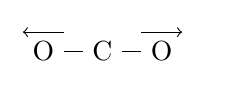
\begin{tikzpicture}
\useasboundingbox (-0.2,-0.2) rectangle (2,0.3);
%\draw (-0.2,-0.2) rectangle (2,0.3);

\draw  (0,0) node (o1) {O};
\draw  (0.75,0) node (c) {C};
\draw  (1.5,0) node (o2) {O};

\draw (o1) -- (c) -- (o2);
\draw[->] (o1.north east) -- (o1.north west);
\draw[<-] (o2.north east) -- (o2.north west);
\end{tikzpicture}
\end{marginfigure}
  $\bar{\nu} = 1337$~cm$^{-1}$. Hierbei ändert sich das Dipolmoment nicht, die Schwingung ist also nicht IR aktiv, wäre im Spektrum also nicht zu sehen.


\item[Asymmetrische Streckschwingung]
\begin{marginfigure}
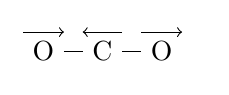
\begin{tikzpicture}
\useasboundingbox (-0.2,-0.2) rectangle (2,0.3);
%\draw (-0.2,-0.2) rectangle (2,0.3);

\draw  (0,0) node (o1) {O};
\draw  (0.75,0) node (c) {C};
\draw  (1.5,0) node (o2) {O};

\draw (o1) -- (c) -- (o2);
\draw[<-] (o1.north east) -- (o1.north west);
\draw[<-] (o2.north east) -- (o2.north west);
\draw[->] (c.north east) -- (c.north west);
\end{tikzpicture}
\end{marginfigure}
 $\bar{\nu} = 2349$~cm$^{-1}$. Hierbei ändert sich das Dipolmoment, die Schwingung ist also  IR aktiv.

\item[Biegeschwingung] 
\begin{marginfigure}
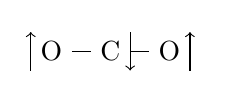
\begin{tikzpicture}
\useasboundingbox (-0.3,-0.2) rectangle (2,0.3);
%\draw (-0.2,-0.2) rectangle (2,0.3);

\draw  (0,0) node (o1) {O};
\draw  (0.75,0) node (c) {C};
\draw  (1.5,0) node (o2) {O};

\draw (o1) -- (c) -- (o2);
\draw[<-] (o1.north west) -- (o1.south west);
\draw[<-] (o2.north east) -- (o2.south east);
\draw[->] (c.north east) -- (c.south east);
\end{tikzpicture}
\end{marginfigure}
 $\bar{\nu} = 667$~cm$^{-1}$. Hierbei ändert sich das Dipolmoment, die Schwingung ist also  IR aktiv. Diese Mode ist zweifach entartet, da sie auch in der Ebene senkrecht zum Papier schwingen könnte. Für die Biegung ist das Potential weicher, die Frequenz daher niedriger als für die Streckung.
\end{description}


\paragraph{Wasser} Ein nicht-lineares Molekül mit $f=9 - 6 = 3$ Schwingungsfreiheitsgraden
\begin{description}
\item[Symmetrische Streckschwingung] 
\begin{marginfigure}
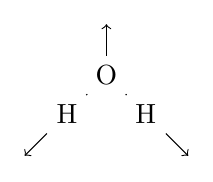
\begin{tikzpicture}
\useasboundingbox  (-0.5,-0.5) rectangle (1.5,1.1);
%\draw (-0.5,-0.5) rectangle (1.5,1.1);

\draw  (0,0) node (h1) {H};
\draw  (0.5,0.5) node (o) {O};
\draw  (1,0) node (h2) {H};

\draw (h1) -- (o) -- (h2);
\draw[->] (h1.south west) -- ++(-135:4mm);
\draw[->] (h2.south east) -- ++(-45:4mm);
\draw[->] (o.north) -- ++(up:4mm);
\end{tikzpicture}
\end{marginfigure}
  $\bar{\nu} = 3657$~cm$^{-1}$. Hierbei ändert sich das Dipolmoment, die Schwingung ist also  IR aktiv.

\item[Symmetrische Streck-Biegeschwingung]
\begin{marginfigure}
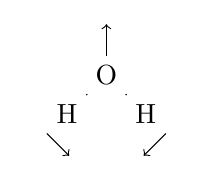
\begin{tikzpicture}
\useasboundingbox  (-0.5,-0.5) rectangle (1.5,1.1);
%\draw (-0.5,-0.5) rectangle (1.5,0.75);

\draw  (0,0) node (h1) {H};
\draw  (0.5,0.5) node (o) {O};
\draw  (1.,0) node (h2) {H};

\draw (h1) -- (o) -- (h2);
\draw[->] (h1.south west) -- ++(-45:4mm);
\draw[->] (h2.south east) -- ++(-135:4mm);
\draw[->] (o.north) -- ++(up:4mm);
\end{tikzpicture}
\end{marginfigure}
  $\bar{\nu} = 1595$~cm$^{-1}$. Hierbei ändert sich das Dipolmoment, die Schwingung ist also  IR aktiv.

\item[Asymmetrische Schwingung]
\begin{marginfigure}
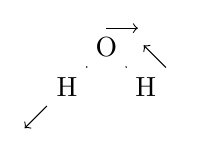
\begin{tikzpicture}
\useasboundingbox  (-0.5,-0.5) rectangle (1.5,0.75);
%\draw (-0.5,-0.5) rectangle (1.5,0.75);

\draw  (0,0) node (h1) {H};
\draw  (0.5,0.5) node (o) {O};
\draw  (1.,0) node (h2) {H};

\draw (h1) -- (o) -- (h2);
\draw[->] (h1.south west) -- ++(-135:4mm);
\draw[->] (h2.north east) -- ++(135:4mm);
\draw[->] (o.north) -- ++(east:4mm);
\end{tikzpicture}
\end{marginfigure}
  $\bar{\nu} = 3756$~cm$^{-1}$. Hierbei ändert sich das Dipolmoment, die Schwingung ist also  IR aktiv.
  
  
\end{description}

\begin{figure}
\inputtikz{\currfiledir fig_hcn-lowres}
\caption{Infrarot-Absorptionsspektrum von HCN Gas  (\cite{Maki_1995_HCN} via \href{https://hitran.org}{hitran.org}). Im unteren Spektrum ist ein größerer Ausschnitt bei geringer Auflösung gezeigt. Hier sind von den Rotationsbanden nur die Einhüllenden zu erkennen.
\label{fig:vib_hcn_all}}
\end{figure}


\paragraph{Cyanwasserstoff (Blausäure, HCN)}  
\begin{marginfigure}
\inputtikz{\currfiledir fig_hcn_modes}
\end{marginfigure}
Ein lineares Molekül mit $f=9 - 5 = 4$ Schwingungsfreiheitsgraden, analog zu Kohlendioxid oben. Das Spektrum in Abb. \ref{fig:vib_hcn} weiter oben zeigt die Biegeschwingung bei $\bar{\nu} = 712$~cm$^{-1}$.  Abbildung \ref{fig:vib_hcn_all} gibt einen Überblick über einen größeren Spektralbereich. Man sieht zusätzlich den 
ersten Oberton der Biegeschwingung bei ungefähr der doppelten Frequenz  $\bar{\nu} = 1415$~cm$^{-1}$. Die Mode bei  $\bar{\nu} = 3312$~cm$^{-1}$ ist die  asymmetrische Streckschwingung. Die symmetrische Streckschwingung  bei $\bar{\nu} = 2114$~cm$^{-1}$.
 Im Gegensatz zu \ch{CO2} bewegt sich in dieser Mode das Kohlenstoffatom ebenfalls, da die Massen von H und N verschieden sind, und sich ansonsten der  Schwerpunkt bewegen würde. Dies macht diese Mode sehr schwach IR-aktiv.  Nur für den Grundton der Biegeschwingung und die  symmetrische Streckschwingung ist der Q-Zweig erlaubt.




%%%%%%%%%%%%%%%%%%%%%%%%%%%%%%%%%%%%%%%%



\section{Zusammenfassung}

\textit{Schreiben Sie hier ihre persönliche Zusammenfassung des Kapitels auf. Konzentrieren Sie sich auf die wichtigsten Aspekte.}

\vspace*{10cm}


%--------------------
\printbibliography[segment=\therefsegment,heading=subbibliography]
